\documentclass[utf8]{frontiersSCNS}
%\documentclass{frontiersSCNS}

\usepackage{url,hyperref,lineno,microtype,subcaption}
\usepackage[onehalfspacing]{setspace}

\linenumbers

%\usepackage{lineno,hyperref}
\usepackage[separate-uncertainty=true,multi-part-units=single,range-phrase= -- ]{siunitx}
\usepackage{color}
%\modulolinenumbers[5]
\usepackage{mhchem}
\usepackage{makecell}
\usepackage{multirow}
\usepackage{booktabs}
\usepackage[flushleft]{threeparttable}
%\usepackage{enumitem}n
%\usepackage{amsmath}
%\usepackage{trackchanges}
%\usepackage{ulem}
%\usepackage{enumerate}
\graphicspath{{Figures/}}



\newcommand{\COMON}{\begin{color}{blue}}
\newcommand{\COMOFF}{\end{color}}

\newcommand{\alon}{\begin{color}{red}}
\newcommand{\aloff}{\end{color}}

\newcommand{\GSon}{\begin{color}{orange}}
\newcommand{\GSoff}{\end{color}}

\newcommand{\CPon}{\begin{color}{green}}
\newcommand{\CPoff}{\end{color}}


%\renewcommand{\emph}{\textit}




\def\keyFont{\fontsize{8}{11}\helveticabold }
\def\firstAuthorLast{Pacheco {et~al.}} %use et al only if is more than 1 author
\def\Authors{Marcus Pacheco\,$^{1,*}$, Alain Plattner\,$^{2}$, Greg Stock\,$^{3}$, Christopher Pluhar\,$^{1}$ and Dylan H. Rood\,$^{4}$}
% Affiliations should be keyed to the author's name with superscript numbers and be listed as follows: Laboratory, Institute, Department, Organization, City, State abbreviation (USA, Canada, Australia), and Country (without detailed address information such as city zip codes or street names).
% If one of the authors has a change of address, list the new address below the correspondence details using a superscript symbol and use the same symbol to indicate the author in the author list.
\def\Address
 {$^{1}$Earth \& Environmental Sciences, California State University, Fresno, Fresno, CA, USA \\
  $^{2,*}$ Geological Sciences, The University of Alabama, Tuscaloosa, AL, USA\\
  $^{3}$ National Park Service, Yosemite National Park, CA, USA
  $^{4}$ Earth Science and Engineering, Imperial College London, London, UK }
% The Corresponding Author should be marked with an asterisk
% Provide the exact contact address (this time including street name and city zip code) and email of the corresponding author
\def\corrAuthor{Department of Geological Sciences, University of Alabama, 201 7th Ave., Tuscaloosa, AL 35487, USA}

\def\corrEmail{amplattner@ua.edu}






\begin{document}

\onecolumn
\firstpage{1}

%\begin{frontmatter}

\title[Royal Arches Meadow rock avalanche]{Age dating and geophysical investigation of the Royal Arches Meadow Rock Avalanche, Yosemite Valley, California}

\author[\firstAuthorLast ]{\Authors} %This field will be automatically populated
\address{} %This field will be automatically populated
\correspondance{} %This field will be automatically populated

\extraAuth{}% If there are more than 1 corresponding author, comment this line and uncomment the next one.
%\extraAuth{corresponding Author2 \\ Laboratory X2, Institute X2, Department X2, Organization X2, Street X2, City X2 , State XX2 (only USA, Canada and Australia), Zip Code2, X2 Country X2, email2@uni2.edu}


%% %% Group authors per affiliation:
%% \author[Marcus]{Marcus Pacheco\corref{cor1}}
%% \address[Marcus]{Earth \& Environmental Sciences, California State University, Fresno}
%% \cortext[cor1]{Corresponding author.}
%% \ead{mvpacheco90@mail.fresnostate.edu}

%% \author[Alain]{Alain Plattner}
%% \address[Alain]{Geological Sciences, University of Alabama}

%% \author[Greg]{Greg Stock}
%% \address[Greg]{National Park Service, Yosemite National Park}

%% \author[Chris]{[Christopher Pluhar}
%% \address[Chris]{Earth \& Environmental Sciences, California State University, Fresno}


\maketitle

\begin{abstract}

Since the retreat of glaciers in Yosemite Valley after the Last Glacial Maximum, rock avalanches have occurred intermittently in Yosemite Valley, California. We investigated the distal portion of the oldest of these, the Royal Arches Meadow rock avalanche, which was partially buried by post-event aggradation of fluvial sediments. Cosmogenic \ce{^{10}Be} exposure ages of boulders on the deposit indicate that the rock avalanche occurred at \SI{16+-0.3}{\kilo a}, \alon Wait, didn't we get different ages in the table? Or is exposure age not the same as how long ago it occurred? Table says \SI{15.5 \pm 1.3}{\kilo a} \aloff immediately after deglaciation and thus prior to most aggradation. The interface between the rock avalanche deposit and the underlying glacialfluvial sediments therefore provides an elevation marker of the valley floor at the time of deposition. To find the depth to this interface, we collected eight Ground Penetrating Radar (GPR) and five Electrical Resistivity Tomography (ERT) profiles across the rock avalanche. Both methods are sensitive to the contrast between the granitic avalanche deposit and the underlying sediments. By constraining ERT inversions with GPR interfaces that are continuous across the profiles, we identified a single interface, interpreted as the basal contact of the rock avalanche, that separates resistive material from conductive material underneath. The elevation of this approximately horizontal interface is \SI{1207.63+-0.95}{\m}, indicating a cumulative aggradation of \SI{\approx 10}{\m} since deglaciation. Based on topographic expression and depth to basal contact, we obtained a lower-end volume estimation of \SI{955000}{\m^3}, nearly three times larger than would be estimated from surface expression alone. Our findings inform reconstruction of the sedimentation history and landscape evolution of Yosemite Valley, and confirm that geophysical methods are valuable tools for investigating rock avalanches.


\tiny
\keyFont{\section{Keywords:}Rock Avalanche, Ground Penetrating Radar, Electrical Resistivity Tomography, Yosemite Valley, Near-surface Geophysics}
%All article types: you may provide up to 8 keywords; at least 5 are mandatory.
                                                                                \end{abstract}

%\linenumbers






\section{Introduction}\label{sec:intro}

Rock avalanches are among the most powerful geologic forces on earth, rapidly eroding huge masses of rock and causing dramatic landscape changes \citep[e.g.][]{evans2006landslides, hovius2006landslide, korup2007giant, hewitt2008legacies}. As a result of their extremely large volumes and associated long runout distances, rock avalanches are also the source of some of the world’s most destructive natural disasters, posing significant hazard and risk in mountainous environments \citep{evans2006landslides}.

Determining rock avalanche volumes is a key aspect of evaluating their hazard, as accurate volumes are needed to establish robust volume-frequency relationships \citep[e.g.][]{evans2006landslides} and are critical components of empirical equations governing rock avalanche mobility \citep[e.g.][]{davies1999runout, bowman2012physical}.  Rock avalanche volumes are usually determined by field investigations or remote sensing methods, though in both cases accurate volumes can be elusive due to the inherent difficulty in establishing accurate deposit extents and thicknesses, cover by more recent debris, or a lack of sufficiently high resolution remote sensing data \citep{hutchinson2006massive}. This situation is exacerbated in cases where rock avalanche deposits are partially buried by post-event sediment aggradation, with an unknown but likely substantial portion of the deposit volume hidden from view.  Older rock avalanches may be particularly susceptible to this condition. Partial burial can lead to an underestimation of volume, and thus inaccurate conclusions about frequency, runout, and overall hazard.

Here we use integrated geophysical imaging methods to investigate the basal contact, thickness distribution, and volume of the Royal Arches Meadow rock avalanche, a \SI{\approx 16}{\kilo a}, partially-buried rock avalanche deposit in Yosemite Valley.




\subsection{Physical Setting}

Yosemite Valley is located in Yosemite National Park in the central Sierra Nevada mountain range of California (Fig.~\ref{RAMRA}A).  Yosemite Valley is approximately \SI{12}{km} long and \SIrange{1}{2}{km} wide, with steep (including vertical to overhanging) cliffs nearly \SI{1}{km} tall.  These cliffs and associated waterfalls offer iconic scenery that draws more than 4 million visitors annually.  The walls of Yosemite Valley are composed of late Cretaceous granitic rocks of the Sierra Nevada batholith \citep{bateman1992plutonism}, primarily granites, granodiorites, and minor diorite. The cliffs in eastern Yosemite Valley, including those adjacent to the Royal Arches Meadow rock avalanche, are comprised of \SI{\approx88}{Ma} Half Dome Granodiorite \citep{peck2002geologic}.



                                   \begin{figure*}
  
  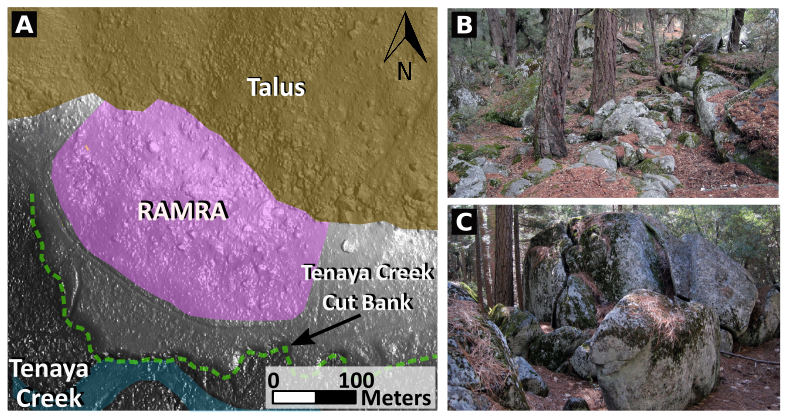
\includegraphics[width=\textwidth]{RAMRA.pdf}
  \caption{ Location and geologic setting of the Royal Arches Meadow rock avalanche.  (A) Location of Royal Arches Meadow rock avalanche in eastern Yosemite Valley, Yosemite National Park (YNP), California (CA).  (B) Oblique topographic hillshade, derived from \SI{1}{m} filtered lidar data, showing the Royal Arches Meadow rock avalanche (blue), adjacent Mirror Lake rock avalanche (green), active talus (brown), and terrace riser adjacent to Tenaya Creek.  Black circles mark samples collected for cosmogenic \ce{^{10}Be} exposure dating.  Extent of oblique view shown as box marked “B” in panel A.  (C) Photograph showing topography typical of the exposed part of the rock avalanche.  (D) Photograph of boulder on the western margin of the rock avalanche sampled for cosmogenic \ce{^{10}Be} exposure dating (sample RAMRA-3). \label{RAMRA}}
        
                                     \end{figure*}



Yosemite Valley was initially carved by river incision, but was subsequently deepened and widened by hundreds of meters during multiple Pleistocene glaciations \citep{matthes1930geologic, huber1987geologic}, mostly recently during the Last Glacial Maximum (LGM). Although the timing of LGM glacier retreat from Yosemite Valley is not precisely known \citep{wahrhaftig2019extent}, results from elsewhere in the Sierra Nevada suggest that LGM deglaciation occurred between \SIrange{18}{16}{\kilo a} \citep[e.g.][]{rood2011chronology, phillips2017glacial}. Glacier retreat left behind a relatively flat valley floor comprised of glacial outwash, lacustrine deposits, and fluvial silts, sands, and gravels \cite[e.g.][]{matthes1930geologic,huber1987geologic}, with several meters of sediment aggradation of the valley floor in the latest Pleistocene and Holocene \cite[e.g.][]{cordes2013supporting,brody2015near}.

Rock slope failures, primarily in the form of rockfalls and rockslides, occur frequently from the glacially-steepened walls of Yosemite Valley \citep{stock2013historical}.  Sheeting (exfoliation) joints in the otherwise massive granite often form rockfall detachment surfaces \citep[e.g.][]{stock2012progressive}.  Smaller rockfalls of hundreds to thousands of cubic meters in volume occur on an annual basis in Yosemite Valley; larger failures up to tens of thousands of cubic meters in volume occur less frequently, but have been documented in the past 150 years \citep{wieczorek2000unusual, stock2013historical, guerin2020quantifying,  zimmer2012rock}.  These events typically have modest runout distances, and their deposition is usually limited to the active talus slopes flanking the base of cliffs.  

However, Yosemite Valley preserves several extremely large boulder deposits up to several million cubic meters in volume, considered to be rock avalanches \citep{matthes1930geologic, wieczorek1999rock, wieczorek2002catastrophic, stock2010catastrophic}.  These deposits extend far beyond the base of active talus slopes onto the valley floor, where they manifest as extensive, low-angle boulder fields.  At least six rock avalanche deposits have been identified in Yosemite Valley, all of which have occurred since LGM deglaciation.  As the floor of Yosemite Valley is wide and flat, and erosion rates of the granitic boulders in the deposits are on the order of tenths of a millimeter per year, these rock avalanche deposits tend to be exceptionally well preserved; the only potentially confounding factor being partial burial by fluvial sediment aggradation.



\subsection{Royal Arches Meadow Rock Avalanche}

The Royal Arches Meadow rock avalanche is located in eastern Yosemite Valley, between a \SI{420}{m}-tall rock tower named Washington Column to the north and Royal Arches Meadow and Tenaya Creek to the south (Fig.~\ref{RAMRA}A).  The portion of the rock avalanche deposit proximal to the cliffs to the north is buried beneath debris from the more recent \SI{\approx 11e6}{m^3} Mirror Lake rock avalanche \citep[][]{wieczorek1999rock, wieczorek2002catastrophic}, as well as aprons of active talus (Fig.~\ref{RAMRA}B).  The distal portion of the deposit has a lobate morphology where it emerges from beneath the overlapping talus, suggesting that it was unconstrained as it spread out southward across the valley floor.  The maximum width of the distal portion is approximately \SI{315}{m}. Contrasting with the relatively steep \SIrange{30}{35}{\degree} repose angles of the active talus slopes, the distal portion of the rock avalanche deposit is nearly flat, sloping only a few degrees to the south.  The deposit has a hummocky morphology and a clast-supported surface cover of angular boulders (Fig.~\ref{RAMRA}C).  Boulders exposed on the surface of the deposit range from tenths of cubic meters to many hundreds of cubic meters in volume, with the largest boulders projecting many meters above the mean deposit surface (Fig.~\ref{RAMRA}D).

Along the southern margins of the rock avalanche deposit, the distribution of boulders on the surface becomes more dispersed, with many meters to tens of meters separating individual boulders.  The intervening surfaces are composed of flat-lying fluvial sediments, and the isolated boulders appear to be embedded within these sediments, suggesting partial burial by fluvial sediments. Farther south, the topography is flat and comprises a fluvial terrace, the edge of which is a \SI{5}{m}-tall terrace riser formed by lateral erosion of Tenaya Creek  (Fig.~\ref{RAMRA}B).  The cutbank consists of layered stratigraphy of silts and sands, with a capping coarse gravel deposit, but does not reveal any rock avalanche debris, indicating that the rock avalanche does not extend in the subsurface as far south as the terrace riser.

Although the morphology of the Royal Arches Meadow rock avalanche clearly indicates that it was sourced from the north wall of Yosemite Valley in the vicinity of Washington Column, an exact source area is not apparent.  A likely explanation for this is that the rock avalanche originated from a cliff that later collapsed entirely, generating the much larger-volume (\SI{\approx 11e6}{m^3}) Mirror Lake rock avalanche \citep{wieczorek1999rock, wieczorek2002catastrophic} and leaving behind a large depression in the valley wall immediately east of Washington Column known as North Dome Gully.  We infer that the source area for the Royal Arches Meadow rock avalanche occurred from a cliff formerly located in the empty space in what is now the North Dome Gully (Fig.~\ref{RAMRA}B).

The ratio of the vertical fall height (H) and the horizontal runout length (L) of rock avalanches, the so called “Fahrboschung”, is commonly used as an index of their mobility \cite[e.g.][]{hsu1975sturzstroms, corominas1996angle}. As the source area of the Royal Arches Meadow rock avalanche is no longer visible, it is not possible to precisely quantify these parameters. However, given the general constraints on the likely source area, we estimate a maximum fall height of approximately \SI{550}{m} and a maximum runout length of approximately \SI{840}{m}, suggesting an H/L ratio of \SI{0.65}.  As with the other rock avalanches in Yosemite Valley \citep{wieczorek1999rock}, the Royal Arches Meadow rock avalanche does not appear to display “excess” runout; rather, its relatively large runout distance compared to the active talus is explained primarily by its potential energy \cite[e.g.][]{brian1998long}.
	
As the proximal portion of the rock avalanche is buried beneath younger talus and rock avalanche debris, we have not attempted to account for that volume. The exposed distal portion of the Royal Arches Meadow rock avalanche has a volume of approximately \SI{378000}{m^3}, calculated by delineating the area of exposed boulders on the surface (\SI{54186}{m^2}) and measuring the volume within this area that projects above the height of the adjacent, roughly planar, valley floor surface (\SI{1217}{m} elevation).  \COMON The distal portion of the rock avalanche has a mean thickness of XX m and a maximum thickness of XX m \COMOFF. Importantly, this volume measurement assumes that the base of the rock avalanche is the modern valley floor surface, and that the entire volume of the distal portion is presently exposed.  However, as described above, there is evidence that the Royal Arches Meadow rock avalanche is partially buried due to post-event sediment aggradation.  Recognition that post-glacial aggradation likely strongly influences the surface expression of the rock avalanche was a primary motivation for integrated geophysical imaging of the deposit.  

                                

\section{Age of the Royal Arches Meadow rock avalanche}\label{sec:age}

The intact deposit of the Royal Arches Meadow rock avalanche on the floor of Yosemite Valley confirms that it must be post-glacial in age.  However, several lines of field evidence, including overlapping deposition by the Mirror Lake rock avalanche and indications of substantial post-depositional aggradation of fluvial sediments adjacent to and within the distal portion of the deposit, suggest that it may be among the oldest of the rock avalanches in Yosemite Valley. To date the Royal Arches Meadow rock avalanche directly, we employed terrestrial cosmogenic \ce{^{10}Be} exposure dating of boulders on the surface of the deposit.

Terrestrial cosmogenic exposure dating, which utilizes the accumulation of cosmogenic nuclides in target minerals with time due to exposure to cosmic rays \citep[e.g.][]{gosse2001terrestrial} offers a robust means of directly dating rock avalanche deposits, provided the exposed boulders were sufficiently shielded within the rock slope prior to failure and that they have not experienced substantial post-depositional burial or erosion.  Cosmogenic exposure dating has been used to constrain the timing of rock avalanches in a variety of settings \citep[e.g.][]{ballantyne2004beinn, mitchell2007keylong, moreiras2015cosmogenic, nagelisen2015post}, and was previously used to obtain ages for two rock avalanches in Yosemite Valley \citep{stock2010catastrophic, cordes2013supporting}.

We collected three samples for cosmogenic \ce{^{10}Be} exposure dating from boulders on the surface of the Royal Arches Meadow rock avalanche deposit.  We selected large boulders near the distal edge of the deposit that were solidly wedged against adjacent boulders (demonstrating that the boulders could not have rotated since emplacement), and sampled the tops of these boulders to simplify the exposure geometries and topographic shielding, and to minimize the potential for nuclide loss due to wildfire-induced boulder spallation. We did not correct for snow shielding. Sample preparation and accelerator mass spectrometer measurements were made at Scottish Universities Environmental Research Centre using standard procedures. Model exposure ages were calculated using the CRONUS-Earth online calculator \citep{phillips2016cronus, marrero2016cosmogenic}.

Results from the three samples are nearly identical (Table~\ref{age}), yielding a mean exposure age of \SI{15.5+-1.3}{\kilo a}.  This result confirms that the Royal Arches Meadow rock avalanche is late Pleistocene in age. Given that the Royal Arches Meadow rock avalanche is located close to the inferred LGM terminus position (within \SI{7}{km}), it is reasonable to assume that deglaciation had occurred there by \SI{\approx 16}{\kilo a}, and that the rock avalanche occurred shortly thereafter.  As such, the Royal Arches Meadow rock avalanche presents an important marker of the position of the floor of Yosemite Valley immediately following deglaciation, providing insights into the post-glacial history of the valley.  As much of this history involved aggradation of fluvial and colluvial sediments adjacent to, and on top of, the rock avalanche, the relationship between the rock avalanche and the former valley floor has been obscured.  We thus turned to geophysical imaging to investigate the position and nature of the basal contact of the rock avalanche deposit.

                            % -Table for RAMRA age here!-
                            
\setlength{\extrarowheight}{4pt}
\renewcommand\arraystretch{1.1}
\begin{table*}
  \caption{Sample data and exposure ages for boulders on the Royal Arches Meadow rock avalanche. \label{age}}
  \vspace*{0.2cm}
%\begin{tabular}{|c|c|c|c|c|c|c|}
%\multicolumn{2}{c|}
\begin{threeparttable}
  \begin{tabular*}{\textwidth}{ccccccc}
    \hline
    \addlinespace[0.1cm]
    Sample & \makecell{Latitude \\ ($^\circ$N)} & \makecell{Longitude \\ ($^\circ$W) } & \makecell{Elevation \\ (m AMSL\tnote{1})} & \makecell{Sample \\  thickness (cm)}  & \multicolumn{2}{c}{\makecell{  \ce{^{10}Be} production rate\\ (\si{atoms \per g \per yr})}} \\
    %\cline{6-7}
    & &&&& Be spallation &  Mu spallation \\
    \hline 
    RAMRA-1 & 37.743351 & -119.56008 & 1224 & 2   & 9.1740 & 0.088505 \\
    RAMRA-2 & 37.743725 & -119.56185 & 1220 & 3   & 8.9742 & 0.087371 \\
    RAMRA-3 & 37.744736 & -119.56255 & 1222 & 2.2 & 9.0503 & 0.087376 \\
    \hline
  \end{tabular*}
  
  
  \vspace{0.5cm}
  %\begin{tabular}{|c|c|c|c|c|c|c|}
  \begin{tabular*}{\textwidth}{ccccccc}
    \hline
    \addlinespace[0.1cm]
    Sample & \makecell{Shielding \\ factor} & \makecell{Mass  \\ ( quartz \si{g})} & \makecell{\ce{Be} carrier\\ (\si{g}) } & \makecell{\ce{^10Be}/\ce{^9Be}\\ ($\times $\num{e13})}& \makecell{\ce{^10Be} concentration \\  ($\times $\SI{e4}{atoms \per g \, \ce{SiO_2}}) } & \makecell{Exposure Age\tnote{2}\\  (\si{\kilo a})}\\
    \hline
    RAMRA-1& 0.929307 & 16.122 & 0.4460 & \num{1.52 \pm 0.04} & \num{12.583 \pm 0.370} & \num{15.5 \pm 1.3} \\
    RAMRA-2& 0.919873 & 17.168 & 0.4462 & \num{1.59 \pm 0.04} & \num{12.366 \pm 0.352} & \num{15.5 \pm 1.3} \\
    RAMRA-3& 0.918220 & 17.999 & 0.4458 & \num{1.69 \pm 0.05} & \num{12.551 \pm 0.368} & \num{15.6 \pm 1.3} \\
    \hline
  \end{tabular*}
  
  \vspace{0.2cm}
  \begin{tablenotes}
  \item[1]
  Metres Above Mean Sea Level. 
  \item[2] 
  Exposure ages calculated using the CRONUS web calculator, version 2.0 \citep{phillips2016cronus, marrero2016cosmogenic}, \url{http://cronus.cosmogenicnuclides.rocks/2.0}, assuming a rock density of \SI{2.7}{g \per cm}, standard atmosphere, a boulder erosion rate of \SI{0.00065}{cm\per yr} \citep{wahrhaftig2019extent}, and using the Lifton-Sato-Dunai scaling scheme \citep{lifton2014scaling}.
  \end{tablenotes}
\end{threeparttable}
\end{table*}
 
\section{Geophysical Investigation}\label{sec:geophys}

We used a combination of two non-intrusive geophysical methods --- Electrical Resistivity Tomography (ERT) and Ground Penetrating Radar (GPR). GPR common-offset profiling consists of keeping transmitter and receiver antennae at a fixed offset and recording traces along a profile line \citep{jol2008ground}. Electromagentic wavelets emitted by the transmitter antenna at each measurement location get reflected by subsurface contrasts in dielectric permittivity \citep{neal2004ground} and recorded by the receiver antenna. A variety of factors including change in lithology, grain size and orientation, and the water table affect the dielectric permittivity \citep{Olhoeft1998,neal2004ground}. This makes GPR a well-suited technique to investigate the interface between the granitic rock avalanche deposit and the underlying valley sediments (lacustrine, deltaic and fluvial). To image the subsurface, signals recorded by the GPR receiver antenna at each position along the profile are plotted next to each other to form a radargram. Since the vertical axis of a radargram shows the time since source wavelet transmission, subsurface radar wave velocity is required to extract depth information. This velocity can be obtained by conducting a ``common midpoint'', or a ``wide angle reflection and refraction'' survey, in which the separation between transmitter and receiver antenna is successively increased \citep{annan1976impulse, davis1989ground}.


In ERT surveys, electrical potential differences arising from electrical current injected into the ground reveal the spatially varying electrical resistivity of the subsurface. Measurements using multiple current- and potential-electrode pairs along a profile allow computer tomographic inversions to create vertical profiles showing the two-dimensional variation of electrical resistivity \citep{oldenburg1999estimating, loke2013recent}. We expected the electrical resistivity of the granitic rock avalanche debris to be an order of magnitude higher than the resistivity of the underlying lacustrine, deltaic and fluvial sediments, posing a strong contrast in the physical parameter to which ERT is sensitive.


Neither of the two methods by itself can pinpoint the the basal contact of the rock avalanche. While GPR shows the boundaries of various units, it is not well suited to differentiate between the unit materials. When several interfaces are present, GPR alone will not conclusively indicate which of these interfaces is the basal contact of the rock avalanche deposit. ERT, on the other hand, is sensitive to the materials of the units, but can not by itself resolve sharp transitions. Moreover, electrical resistivity tomography is typically underdetermined, meaning that different resistivity profiles may fit the data equally well. As a consequence, additional constraints (regularization) must be provided, typically in the form of imposed smoothness \citep[e.g.][]{gunther2006three, loke2013recent}. As a result, different regularization constraints may lead to different resistivity profiles \citep{oldenburg1999estimating}. A-priori information of subsurface structure can be incorporated into ERT regularization. Here, we follow the approach of \cite{doetsch2012constraining} by removing smoothing constraints across interfaces obtained from GPR profiles that overlap with our ERT profiles.

Previous studies in the Austrian Alps and Bavarian Alps \citep{sass2006determination, sass2001investigations}, the Swiss Alps \citep{otto2006comparing, socco2010geophysical}, and in Yosemite Valley \citep{brody2015near, Liu2018nearAGU} showed the potential of geophysical methods including ERT, GPR, and seismic refraction in studying mass wasting deposits. Here, we decided against using seismic refraction because we expect the seismic velocity of the underlying sediments to be lower than the seismic velocity of the rock avalanche. Such a setting would refract the seismic waves away from the surface and would not allow us to image the basal contact of the rock avalanche.


\subsection{Acquisition Strategy}



We collected eight GPR and five ERT profiles (Fig.~\ref{GPR_ERT_Map} A and B) crossing exposed parts of the rock avalanche as well as the adjacent area covered by finer sediments. GPR profiles as well as ``Wide Angle Reflection and Refraction'' (WARR) data were acquired using a Sensors \& Software PulseEKKO Pro (\SI{50}{\mega Hz}) system between September and October 2018. The five ERT transects were collected in March 2018 with an Advanced Geosciences Inc SuperSting R1 system with 28 electrodes and a \SI{6}{m} electrode spacing, using Schlumberger and dipole-dipole electrode arrays. To increase the length of the ERT profiles, we used a roll-along strategy. ERT and GPR profiles overlapped to allow for joint processing and interpretation. 




								 \begin{figure*}

	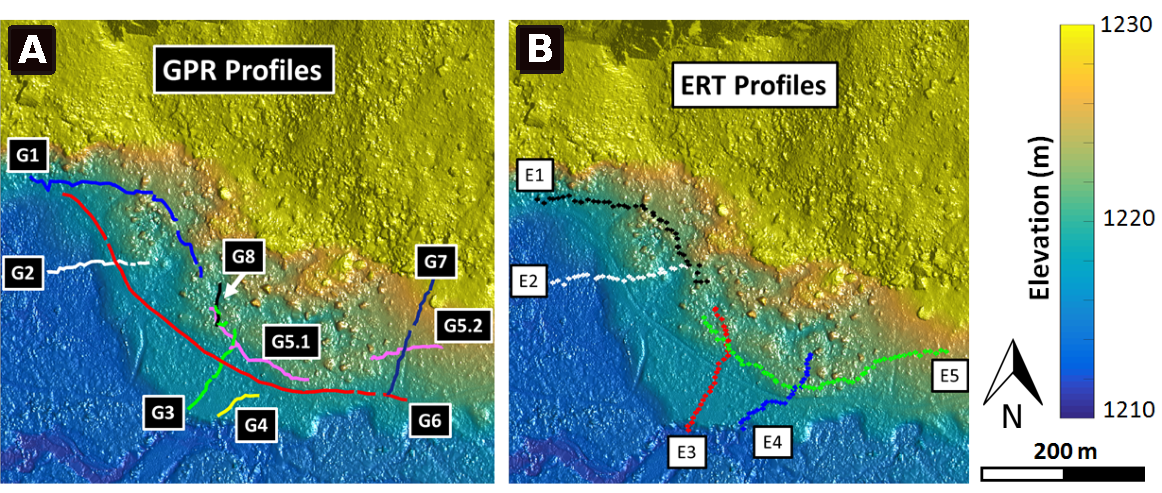
\includegraphics[width=\textwidth]{Figures/GPR_ERT_Map.pdf}
		\caption{:(A) Map view of GPR profiles and WARR location. (B) map view of ERT profiles. GPR and ERT profiles overlap to allow for joint processing and interpretation.  \label{GPR_ERT_Map}}
		
								   \end{figure*}






\subsection{Radar Wave Velocity}\label{GPRvel}

To determine the subsurface velocity, we collected ``Wide Angle Reflection and Refraction'' (WARR) data by transmitting and recording signals at increasing transmitter-receiver separation. The resulting radargram (Fig.~\ref{WARR}C), obtained after minimal processing using GPRPy \citep{plattner2019comunity,plattner2020GPRPy} shows signals traveling directly from the transmitter to the receiver through air (air wave) and through the ground (ground wave) as straight lines, while signals reflected from horizontal interfaces appear as hyperbolae. The slope of the direct arrivals and the shape of the hyperbolae allow us to determine the subsurface velocity. We used the stacked amplitude procedure implemented in GPRPy to give best estimations for direct waves (Fig.~\ref{WARR}B) and reflected waves (Fig.~\ref{WARR}A). As expected, the air wave traveled at the speed of light in air (\SI{0.3}{ns \per m}). The ground wave samples only the shallowest part of the subsurface its velocity is hence not necessarily representative of the deeper subsurface. The reflected arrivals (hyperbolae), on the other hand, travel down to the interface and hence provide an estimation for the average subsurface velocity between the interface and the surface. We therefore use the velocity obtained from the hyperbolae, \SI{0.11}{m \per ns}, as subsurface velocity.



	                                 \begin{figure*}

	\includegraphics[width=\textwidth]{Figures/WARR.pdf}
		\caption{:(A) hyperbolic stacked amplitudes for the WARR data in Fig.~\ref{WARR}C. Bright colors indicate velocities and depths (two-way travel time) of interfaces. (B) linear stacked amplitudes for the WARR data in Fig.~\ref{WARR}C. Bright colors indicate velocities for direct waves. (C) WARR data with best-fitting lines and hyperbolae obtained from Fig.~\ref{WARR}A~and~B.\label{WARR}}
		
		                        	   \end{figure*}



\subsection{GPR Data Processing and interpretation}

Minimal GPR data processing using GPRPy \citep{plattner2019comunity,plattner2020GPRPy} included a time-zero correction, filter (dewow and mean trace removal), T-power gain, f-k migration \citep{stolt1978migration} and topographic correction. Processing scripts including the parameters used in the processing are provided together with the raw data. For the time-to-depth transformation, we used a homogeneous velocity of \SI{0.11}{m \per ns} obtained from a WARR survey (Section~\ref{GPRvel}) \citep{annan1976impulse, davis1989ground}. 

To identify candidates for the basal contact of the rock avalanche in the processed GPR data, we plotted the GPR profiles in their three-dimensional context (Fig.~\ref{GPR_Oblique}) and identified interfaces that are consistent between the profiles and continue underneath the exposed rock avalanche as well as the surrounding area. We identified three candidates for the basal contact (Fig.~\ref{GPR_Oblique}B): A relatively flat interface (parallel to the surface) ``\emph{Alpha}'' ranging between \SI{1216}{m} and \SI{1214}{m} above mean sea level, a deeper, nearly-horizontal interface ``\emph{Beta}''  at an elevation of \SI{1207.63 \pm 0.95}{\m} (Fig.~\ref{GPR_Oblique}C), and ``\emph{Gamma}'', which is visible in profiles G2 -- G7 at an elevation of \SI{\approx 1205}{m}. Between interface \emph{Alpha} and \emph{Beta}, we observe scattering that is more prominent than below interface \emph{Beta} (Fig.~\ref{GPR_Oblique}B). Uncertainty in our velocity assessment influences the accuracy of the inferred interface elevations. For interface \emph{Beta}, a velocity range of \SI{0.108}{m \per ns} to \SI{0.124}{m \per ns} leads to an elevation range of \SI{1207.17}{m} to \SI{1207.98}{m}.



								 \begin{figure*}

	\includegraphics[width=\textwidth]{Figures/GPR_Oblique.pdf}
		\caption{:(A) Oblique view of GPR profiles looking towards NW, (B) Identified interfaces \emph{Alpha}, \emph{Beta}, and \emph{Gamma}, and (C) Interpolated surface for interface \emph{Beta}. \label{GPR_Oblique}}

								   \end{figure*}

							   
			   

								   
\subsection{GPR-constrained ERT inversion}

To identify which of the previously found candidates is the basal contact of the rock avalanche, we removed smoothing constraints across interface \emph{Alpha}, \emph{Beta}, and \emph{Gamma} in the ERT inversion of the corresponding profiles \citep{doetsch2012constraining} using the open-source software BERT \cite[][]{gunther2006three,Ruecker2017}. This  approach does not enforce but allows sharp transitions across the provided interface. We use profile E3 to illustrate the process (Fig.~\ref{ERT_inversion}), but other profiles showed a similar pattern. For a granitic debris deposit overlying lacustrine, deltaic and fluvial sediments, we expected electrically resistive material on top of conductive material. Indeed, inversion of the resistivity data with regular smoothing and no additional a-priori constraints revealed electrically resistive material (\SI{> 5000}{\ohm m}) overlying relatively conductive material (\SI{< 1000}{\ohm m}), but with a smooth transition (Fig.~\ref{ERT_inversion}A). For interface \emph{Alpha}, resistive material is still present below the interface (Fig.~\ref{ERT_inversion}B). Interface \emph{Beta} created a sharp transition between resistive and conductive material (Fig.~\ref{ERT_inversion}C). Interface \emph{Gamma} lies below the transition of resistive to conductive material for most of the profile (Fig.~\ref{ERT_inversion}D). 




							 \begin{figure*}

	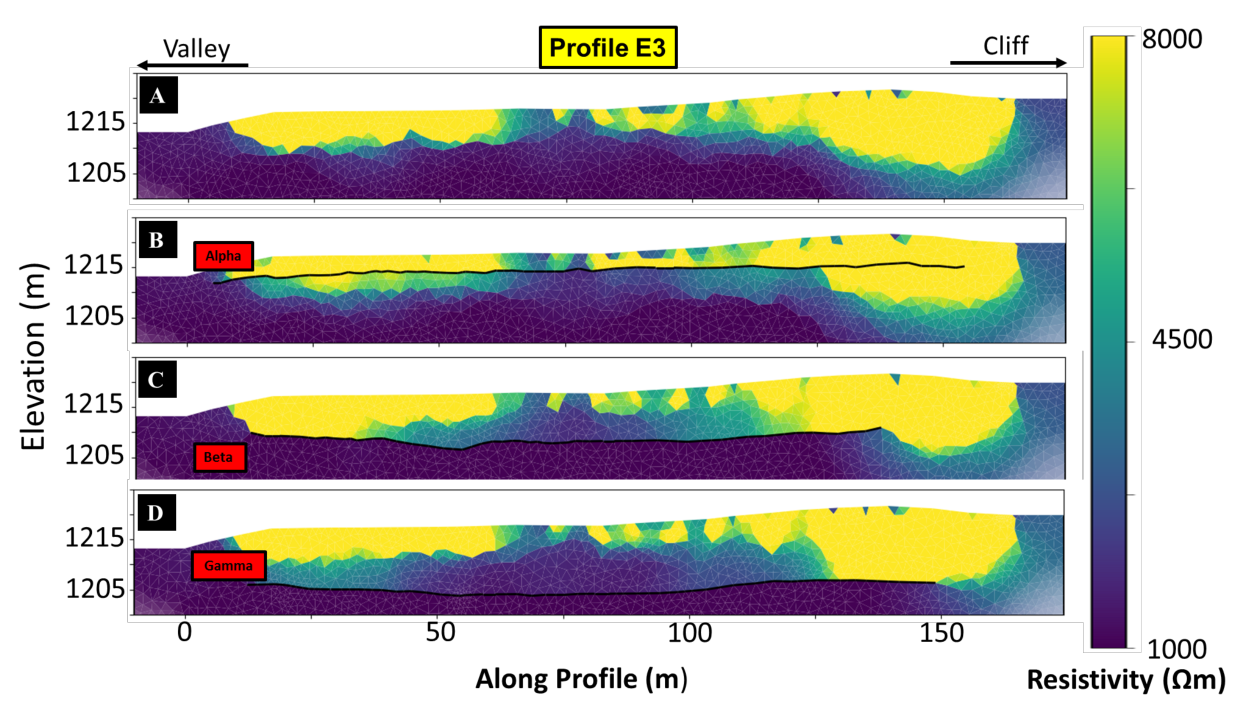
\includegraphics[width=\textwidth]{Figures/ERT_inversion.pdf}
		\caption{ERT inversion results for profile E3 using smoothness regularization. (A) No additional a-priory information, smoothness applied everywhere. (B) No smoothing across interface \emph{Alpha}, (C) no smoothing across interface \emph{Beta}. (D) No smoothing across interface \emph{Gamma}.\label{ERT_inversion}}

								   \end{figure*}

Identifying \emph{Alpha}, \emph{Beta}, and \emph{Gamma} underneath the rugged terrain of the exposed rock avalanche was more challenging than underneath the adjacent smooth terrace. Interfaces in GPR profile G5.1 (Fig.~\ref{Combined_ABCD}A) are less clear than in profiles G3 and G6 (Fig.~\ref{GPR_Oblique}). In profile G5.1, we identified interfaces (Fig.~\ref{Combined_ABCD}B) at elevations of \SI{\approx 1216}{m} (\emph{Alpha}), \SI{\approx 1213}{m} (unnamed), and \SI{\approx 1207}{m} (\emph{Beta}). Interface \emph{Gamma} is not visible in this GPR profile. Similar to the GPR-constrained ERT inversion for profile E3 (Fig.~\ref{ERT_inversion}), interface \emph{Beta} creates the clearest separation between resistive and conductive materials (Fig.~\ref{Combined_ABCD}C,~D).  

                                \begin{figure*}

	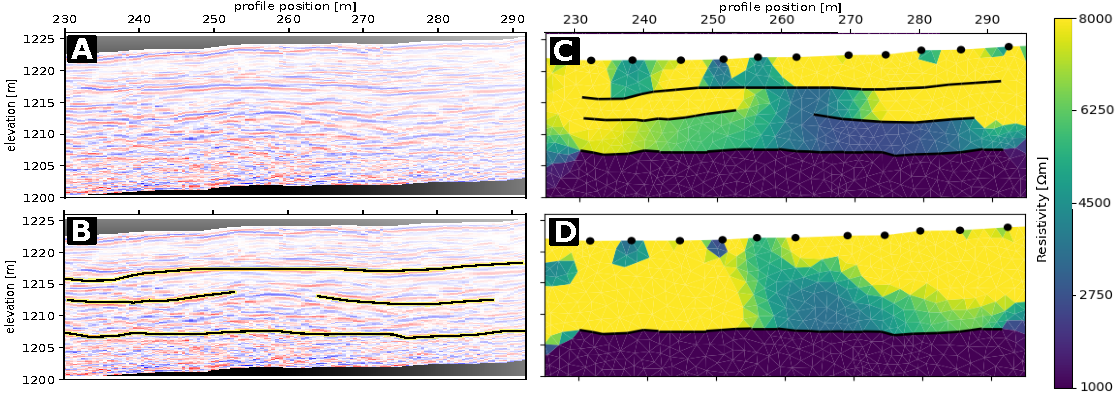
\includegraphics[width=\textwidth]{Figures/Combined_ABCD.pdf}
		\caption{(A) GPR profile G5.1. (B) Profile G5.1 with marked interfaces. (C) GPR-constrained ERT inversion result using all marked interfaces. (D) GPR-constrained ERT inversion result using only interface \emph{Beta}. \label{Combined_ABCD}}

								   \end{figure*}


\section{Results and Implications}\label{sec:results}

We identified \emph{Beta} as the interface between the rock avalanche deposit and the underlying sediments, which we interpret as the paleo-surface of Yosemite Valley shortly before the rock avalanche event. Our choice of \emph{Beta} is based on the following observations.

\begin{enumerate}
\item Of all three interfaces identified in the GPR data, \emph{Beta} led to the clearest separation between electrically resistive and conductive material in GPR-constrained ERT inversions (Fig.~\ref{ERT_inversion},~\ref{Combined_ABCD}).
\item In the GPR data, \emph{Beta} separates a unit of visible scattering from a unit with little scattering underneath (Fig.~\ref{GPR_Oblique}). We interpret that the scattering of radar waves is a result of randomly oriented granite clasts. 
\end{enumerate}


\subsection {Rock avalanche subsurface Volume}

Assuming that the edge of the distal surface expression of the rock avalanche coincides with its lateral extent and  that the basal contact of the rock avalanche is level and flush with the edge of the exposed portion of the rock avalanche (\SI{\approx 1217}{m} AMSL) yields a volume of \SI{\approx 378000}{m^3}. However, our results indicate a deeper basal contact at \SI{\approx 1207}{m} AMSL. Identifyying the lateral edge of the rock avalanche proved to be challenging, as it overlapped with talus deposits. Here we provide an updated \emph{lower-limit estimate} for the volume of the Royal Arches Meadow rock avalanche. Using the lateral extent of the exposed portion of the rock avalanche deposit, but with a basal contact elevation of \SI{1207}{m} AMSL yields a minimum volume of \SI{\approx 955000}{m^3}, an increase of a nearly a factor of three compared to the previous lower-bound estimation. Correcting for an assumed 25\% porosity of the rock avalanche deposit \cite[e.g.'][]{hutchinson2006massive, stock2010catastrophic} leads to a minimal intact rock volume of approximately \SI{668500}{m^3}. Since this is a lower-limit estimation, the actual volume is likely larger.


\section{Conclusions}\label{sec:conclusions}

\ce{^{10}Be} exposure dating revealed that the Royal Arches Meadow rock avalanche occurred \num{15.5+-1.3}~thousand~years ago, shortly after deglaciation of the eastern Yosemite Valley. We identified the basal contact of the Royal Arches Meadow rock avalanche in Yosemite Valley at an elevation of \SI{1207}{m} above mean sea level using a combination of ERT and GPR data. The adjacent terrace has a surface elevation of \SI{1217}{m} AMSL, indicating a \SI{10}{m} cummulative aggradation over \num{\approx 15000} years. We estimate the volume of the Royal Arches Rock avalanche deposit to be at least \SI{955000}{m^3}, but likely significantly larger. Talus deposits and sediment cover impeded identifying the lateral extent of the rock avalanche deposit. 






\section*{Conflict of Interest Statement}
The authors declare that the research was conducted in the absence of any commercial or financial relationships that could be construed as a potential conflict of interest.


\section*{Author Contributions}
All authors discussed the results and contributed to the manuscript. MP collected and processed the geophysical data. AP collected ERT data and served as faculty advisor to MP. GS collected and processed the \ce{^{10}Be} age data. 

\alon Everyone, please check and adapt this statement. \aloff

\alon
The Author Contributions section is mandatory for all articles, including articles by sole authors. If an appropriate statement is not provided on submission, a standard one will be inserted during the production process. The Author Contributions statement must describe the contributions of individual authors referred to by their initials and, in doing so, all authors agree to be accountable for the content of the work. Please see  \href{http://home.frontiersin.org/about/author-guidelines#AuthorandContributors}{here} for full authorship criteria.
\aloff

\section*{Funding}
This material is based upon work supported by the National Science Foundation under Grant No. EAR-1550732

\alon 
[ The mentioned grant is used to pay Marcus for the summer and some of my time to work on this paper. Greg, do you or your coauthor have grants to mention here?]

Details of all funding sources should be provided, including grant numbers if applicable. Please ensure to add all necessary funding information, as after publication this is no longer possible.
\aloff

\section*{Acknowledgments}

Jessica Thompson-Jobe assisted with sampling for cosmogenic exposure dating.  We appreciate helpful discussions with Elizabeth Haddon and Brendon Quirk. We are thankful for the geophysical fieldwork help provided by Guohai Jia, Jukya and Ryuya Kimura, Mathieu Richaud, Amalie Larsen, and Jessie Shields. 

% \section*{Supplemental Data}
% \alon
% Need to figure this one out. I don't think we want to put all data and scripts as supplemental material. Maybe rather make them available in an online repository and provide a DOI in the data availability statement?

% What other material would go here?

%  \href{http://home.frontiersin.org/about/author-guidelines#SupplementaryMaterial}{Supplementary Material} should be uploaded separately on submission, if there are Supplementary Figures, please include the caption in the same file as the figure. LaTeX Supplementary Material templates can be found in the Frontiers LaTeX folder.
% \aloff

\section*{Data Availability Statement}
The geophysical datasets generated and analyzed for this study can be found on \url{https://github.com/NSGeophysics/RAMRA_Data} (doi: 10.5281/zenodo.3732464).


\bibliographystyle{frontiersinSCNS_ENG_HUMS}
\bibliography{mybibfile}

\end{document}
